\lstset{style=GDS}


\chapter{Metodología} \label{03_Metodología}

En este capítulo se detalla el proceso de diseño e implementación del simulador volumétrico de incendios forestales. A lo largo del mismo, se justificará la elección del entorno de desarrollo, se desglosará la arquitectura del autómata celular y la implementación de los shaders necesarios, se explicará la integración de datos topográficos reales para la generación del terreno y, finalmente, se comentarán los mecanismos de interacción desarrollados y los principales retos arquitectónicos encontrados.
\section{Selección de herramientas}

La selección del entorno de desarrollo es una decisión importante que afecta al rendimiento y la escalabilidad del proyecto. A diferencia de otros software, un simulador de incendios forestales en tiempo real basado en autómatas celulares necesita procesar una gran cantidad de datos topográficos y realizar numerosos cálculos para su correcto funcionamiento.\\

Es por esto que la decisión no se ha basado en las capacidades de renderizado fotorrealista del motor, sino en los siguientes requisitos técnicos:
\begin{itemize}
    \item \textbf{Capacidad de cómputo en paralelo.} Para simular la propagación del fuego a través de la matriz volumétrica es necesario que tenga soporte para la ejecución de \textit{Compute Shaders} permitiendo actualizar el estado de miles de celdas en tiempo real sin saturarse.
    
    \item \textbf{Control sobre la memoria VRAM.} Es necesario disponer de un gran control de la memoria de video para gestionar los buffers de datos y la sincronización para la comunicación entre la GPU y la CPU sin ocasionar cuellos de botella.
    
    \item \textbf{Gestión dinámica de datos geoespaciales.} Para el funcionamiento, los datos que se introducirán son Modelos Digitales de Elevaciones (DEM) y mapas de clasificación de vegetación, por lo que es necesario que se proporcionen interfaces que faciliten su manipulación y conversión a estructuras 3D.

    \item \textbf{Curva de aprendizaje y ecosistema desacoplado.} El entorno debe proporcionar una interfaz clara con una buena documentación, además de una estructura modular que permita separar de forma lógica las distintas interfaces de las que dispondrá el simulador.
    
\end{itemize}

\subsection{Comparativa de motores gráficos}

Para el desarrollo de este simulador, la elección del motor gráfico se ha basado en los requisitos tecnicos mencionados anteriormente, evaluando los tres motores de desarrollo con mayor cuota de mercado y soporte de la industria:


\begin{itemize}
    \item \textbf{Unreal Engine:} Es el motor líder en fidelidad gráfica y rendimiento ofreciendo un control de bajo nivel mediante C++. Sin embargo, para la implementación de \textit{Compute Shaders} necesita una gran cantidad de código de configuración ya que su arquitectura está fuertemente acoplada a su propio \textit{pipeline} de renderizado. En cuanto a portabilidad, aunque es el estándar para consolas de última generación y entornos Windows, la compilación cruzada hacia Linux o macOS suele necesitar configuraciones del entorno muy pesadas, mientras que para plataformas móviles genera aplicaciones con una huella de memoria enorme además de haber descontinuado oficialmente su soporte nativo para exportación web (HTML5).

    \item \textbf{Unity:} Es una de las herramientas más versátiles del mercado y cuenta con soporte nativo para la ejecución de \textit{Compute Shaders} en HLSL. Pero tiene ciertas limitaciones para esta simulación, al depender de un recolector de basura (\textit{Garbage Collector}), que provoca picos de latencia al transferir grandes matrices de datos entre la CPU y la GPU. A nivel de portabilidad, Unity destaca históricamente por su robustez para exportar proyectos para los  sistemas operativos mas usados y sistemas móviles, no obstante aunque permite compilar para navegadores web mediante WebGL, genera \textit{builds} con un gran tamaño base que repercuten negativamente en los tiempos de carga en entornos no especializados. 

    \item \textbf{Godot:} Es un motor de código abierto con licencia MIT. A partir de su version 4.X ha integrado la API Vulkan la cual resulta muy determinante ya que contiene la interfaz \texttt{RenderingDevice}, que permite un acceso directo de bajo nivel a la GPU. Esto permite compilar y ejecutar \textit{Compute Shaders} (escritos en GLSL puro) con un control absoluto sobre la memoria VRAM y los \textit{buffers} de datos. A nivel de portabilidad, Godot destaca por su excepcional agilidad: su propio editor permite compilar ejecutables nativos para Windows, Linux, macOS, Android e iOS en cuestión de segundos y sin requerir pesados compiladores externos ni dependencias adicionales.También es relevante su optimizado soporte para la plataforma web (HTML5/WebAssembly), generando binarios extremadamente ligeros.

\end{itemize}

\begin{table}[H]
    \centering
    \small
    \renewcommand{\arraystretch}{1.5}
    \noindent\makebox[\textwidth][c]{
        \begin{tabular}{|p{3.5cm}|p{3.8cm}|p{3.8cm}|p{3.8cm}|}
            \hline
            \textbf{Característica} & \textbf{Godot 4} & \textbf{Unity} & \textbf{Unreal Engine 5} \\ \hline
            
            \textbf{Soporte \textit{Shaders}} & Óptimo \newline (Nativo GLSL) & Bueno \newline (Nativo HLSL) & Complejo \newline (Abundante configuración C++) \\ \hline
            
            \textbf{Acceso VRAM} & Directo \newline (\texttt{RenderingDevice}) & Intermediado \newline (\textit{ComputeBuffers}) & Abstraído \newline (\textit{Render Graph}) \\ \hline
            
            \textbf{Portabilidad (S.O.)} & Ágil e integrada \newline (Compilación cruzada directa sin dependencias externas) & Buena \newline (Requiere pesados módulos anclados al sistema) & Enfocada a consolas/Windows, herramientas de compilación pesadas \\ \hline

            \textbf{Exportación Web} & Excelente \newline (Binarios ligeros y carga rápida en HTML5/WASM) & Funcional \newline (\textit{Runtime} muy pesado, largos tiempos de carga) & Descontinuada  \\ \hline

            \textbf{Lenguajes de desarrollo} & GDScript, C++, C\#, GLSL & C\#, HLSL & C++, Blueprints, HLSL \\ \hline

            \textbf{Arquitectura de software} & Sistema de Nodos \newline (Orientado a la composición jerárquica) & Entidad-Componente \newline (\textit{MonoBehaviours} / ECS) & \textit{Actors} y Componentes \newline (Acoplado al núcleo central) \\ \hline

            \textbf{Huella del entorno } & Ultra ligero \newline (Unos 100 MB, editor autónomo y portable) & Pesado \newline (Varios GBs, dependiente del \textit{Unity Hub}) & Muy pesado \newline (Mas de 30 GBs de base estructural) \\ \hline
            
            \textbf{Sobrecarga (\textit{Overhead})} & Muy baja \newline (Estable en tiempo real) & Media \newline (Picos de latencia por \textit{G. Collector}) & Muy alta \newline (Decenas de servicios en segundo plano) \\ \hline
            
            \textbf{Licencia} & MIT \newline (Libre y código abierto) & Privada \newline (Suscripción o tarifa por ingresos) & Privada \newline (Regalías por ingresos brutos) \\ \hline
        \end{tabular}
    }
    \caption[Comparativa técnica de motores gráficos]{Comparativa técnica de los motores gráficos evaluados frente a los requisitos arquitectónicos y de despliegue del simulador.}
    \label{tab:comparativa_motores}
\end{table}
\clearpage

Llevando a cabo un análisis de todas estas características de los diferentes entornos de desarrollo y teniendo en cuenta que el núcleo del proyecto implica una comunicación constante, masiva y de bajísima latencia con la GPU, se llega a la conclusión de que Godot es la mejor opción. Dicho entorno resuelve esta necesidad a través de la API \texttt{RenderingDevice} de Vulkan, ofreciendo un control de memoria que esquiva la sobrecarga estructural de Unreal y la recolección de basura de Unity. Además, a esto se le suma un \textit{overhead} mínimo y una portabilidad que, comparada con los otros motores, resulta excepcional permitiendo compilar binarios ultraligeros y de despliegue directo tanto en sistemas de escritorio como en entornos web. Todo ello bajo una licencia de código abierto (MIT) ideal para la investigación científica, que consolida finalmente a Godot como la infraestructura tecnológica más eficiente, versátil y racional para afrontar los retos técnicos de este simulador.\\


\section{Arquitectura del Simulador}
    El disño de la arquitectura de este proyecto se ha dirigido con la necesidad de tratar de manera eficiente una simulación con un gran volumen de datos. Para ello, se ha establecido un modelo de procesamiento híbrido donde la CPU se encarga la lógica de control y la administración del flujo de la aplicación mientras que la GPU actúa como motor físico para ejecutar el cálculo masivo en paralelo. A lo largo de esta sección se explicará cada uno de los componentes de esta arquitectura, desde los fundamentos tecnológicos para su correcta compresión hasta la implementación técnica en la GPU y sincronización de memorias.  

    \subsection[\textit{Pipeline} Gráfico]{Fundamentos tecnológicos: Arquitectura de la GPU y el \textit{Pipeline} Gráfico Tradicional}
        
        Para comprender la base computacional de este simulador, es necesario entender primero la diferencia arquitectónica fundamental entre un procesador central (CPU) y una tarjeta gráfica (GPU). La CPU está diseñada bajo un paradigma de baja latencia, por lo que posee un número reducido de núcleos muy complejos y veloces, optimizados para ejecutar instrucciones secuenciales, saltos lógicos condicionales y administrar el sistema operativo.\\
        
        Por el contrario, la GPU está diseñada para lograr un alto rendimiento, lo que conlleva a su arquitectura a usar un mayor número de núcleos pero siendo la complejidad de cada uno de ellos mucho menor. Una gráfica moderna está compuesta por miles de pequeñas Unidades Aritmético-Lógicas (ALUs) diseñadas para ejecutar la misma instrucción matemática sobre múltiples datos de forma simultánea. Esta estructura le proporciona un paralelismo que es  ideal para procesar gráficos ya que calcular el color de un píxel en la pantalla es independiente del cálculo del píxel adyacente\cite{foley2014computer}.\\

        Para alimentar de datos a estos miles de núcleos simultáneamente sin generar cuellos de botella, la GPU cuenta con su propia memoria, la \textbf{VRAM} (\textit{Video Random Access Memory}). Esta memoria, a diferencia de la memoria RAM administrada por la CPU, posee un ancho de banda masivo diseñado específicamente para operaciones de lectura y escritura altamente paralelas.\\
        
        En el contexto del renderizado visual tradicional la VRAM se organiza en buffers que deben estar estrictamente formateados en estructuras muy específicas, destacando\cite{escudero2023}\cite{referencia_mpg}:
        \begin{itemize}
            \item \textbf{\textit{Vertex Buffers} (VBO):} Almacenan los atributos matemáticos de los vértices que componen una malla 3D, No solo guardan las coordenadas espaciales, sino también datos acoplados a cada vértice, como los vectores normales.
            \item \textbf{\textit{Index Buffers} (EBO/IBO):} Este buffer almacena  únicamente una lista de índices enteros que indica a la GPU en qué orden exacto debe conectar los vértices previamente cargados para generar la malla 3D.
            \item \textbf{\textit{Buffers} de Texturas:} Son estructuras de memoria bidimensionales (y en ocasiones tridimensionales) altamente optimizadas por hardware para el muestreo espacial. Normalmente solo contienen los mapas de color (albedo), rugosidad o desplazamiento aplicados sobre la geometría.
        \end{itemize}

        Históricamente, para aprovechar la potencia de los núcleos y procesar estos \textit{buffers}, los datos debían atravesar un flujo de trabajo unidireccional el cual consta de varias etapas secuenciales para convertir los datos tridimensionales en una imagen 2D:
        
        \begin{enumerate}
            \item \textbf{Ensamblaje de entrada (\textit{Input Assembler}):} La GPU recibe desde la CPU los datos crudos de los modelos 3D (vértices, normales, coordenadas UV).
            \item \textbf{\textit{Vertex Shader}:} Un programa ejecutable que transforma las coordenadas 3D locales de los vértices a las coordenadas 2D de la pantalla de la cámara.
            \item \textbf{Rasterización:} El hardware matemático toma los triángulos formados por los vértices y  determina qué píxeles de la pantalla (fragmentos) están cubiertos por dicha geometría.
            \item \textbf{\textit{Fragment Shader}:} Un segundo programa que calcula el color final, la iluminación y las sombras para cada uno de esos fragmentos.
            \item \textbf{Fusión de salida (\textit{Output Merger}):} Se combinan los fragmentos procesados y se envían al monitor para mostrar la imagen final.
        \end{enumerate}

      
    \subsection[\textit{Pipeline} de Cómputo]{Fundamentos tecnológicos: El \textit{Pipeline} de Cómputo}

        Antes de abordar la solución computacional, es preciso definir formalmente qué es un \textit{shader}, y no es más que un programa diseñado específicamente para ser compilado y ejecutado directamente en los núcleos de la GPU. En motores como Godot, estos \textit{shaders} tradicionales se construyen usando un lenguaje de alto nivel propio (\textit{Godot Shading Language}), el cual abstrae gran parte de la configuración de bajo nivel y está optimizado para integrarse de manera fluida con el motor de renderizado\cite{godot_engine}.\\

        Sin embargo, para el desarrollo de un simulador volumétrico basado en autómatas celulares se necesita actualizar el estado de miles de celdas en cada iteración. Hacer esto de forma secuencial en la CPU generaría un cuello de botella inmenso lo que lo hace inviable para una simulación en tiempo real, y utilizar los \textit{shaders} visuales de Godot obligaría a empaquetar datos matemáticos como si fueran colores. \\
    
        Este problema se ha resuelto haciendo uso del paradigma GPGPU (\textit{General-Purpose computing on Graphics Processing Units}), que consiste en dejar de usar la tarjeta gráfica de forma exclusiva para la visualización y pasar a usarla como un coprocesador matemático masivamente paralelo aplicable a cualquier ámbito. En la práctica, este paradigma permite emplear la enorme cantidad de unidades aritmético-lógicas (ALUs) de la GPU para resolver operaciones matemáticas de propósito general de forma paralela, desligándose por completo del renderizado de imágenes y de las restricciones del \textit{Pipeline} Gráfico tradicional\cite{gpugems3_ch30}.\\

        Esto se ha hecho posible gracias a dejar de usar los shader tradicionales(Vertex y Fragment) para pasar a usar \textbf{\textit{Compute Shaders}} los cuales, a diferencia de los tradicionales, operan de forma independiente al \textit{pipeline} gráfico.Esta independencia les permite usar y estructurar los distintos \textit{buffers} de memoria que necesiten haciéndolos ideales para inyectar los datos topográficos del terreno, calcular la propagación del fuego sobre la matriz del autómata celular en paralelo, y almacenar los resultados térmicos actualizados directamente en la VRAM sin necesidad de someter los datos a un proceso de dibujo en pantalla\cite{gpugems_ch38}.\\

    \subsection{El motor de Simulación}
        \subsubsection*{Elección del modelo}
        La simulación computacional de la propagación de un incendio forestal es un problema matemático complejo que exige traducir procesos físicos y termodinámicos a algoritmos eficientes. En el ámbito de la ingeniería de software aplicada a la predicción de incendios, existen dos grandes enfoques arquitectónicos para modelar el crecimiento del frente de llamas: los modelos vectoriales y los modelos discretos.\\

        Los \textbf{modelos vectoriales}, como ya se ha comentado con anterioridad, representan el avance del fuego como una serie de curvas geométricas que crecen a lo largo del tiempo siguiendo el Principio de Huygens\cite{enders2009huygens}. Los ejemplos más destacados de este enfoque son simuladores profesionales como \textbf{FARSITE} (desarrollado por el Servicio Forestal de EE.UU.) o el sistema canadiense \textbf{Prometheus}.
        \begin{itemize}
            \item \textbf{Ventajas:} Ofrecen una alta precisión espacial y al trabajar con vectores, generan frentes de propagación suaves y visualmente muy realistas, evitando formas cuadriculadas.
            \item \textbf{Desventajas:} Su principal debilidad radica en la resolución topológica ya que cuando dos frentes de fuego colisionan, calcular la intersección matemática de sus polígonos para fusionarlos en una nueva curva requiere algoritmos de geometría secuenciales. Esta dependencia estructural los convierte en un enorme cuello de botella para la paralelización masiva en la GPU.
        \end{itemize}

        Por otro lado, los \textbf{modelos discretos} renuncian a la exactitud del espacio vectorial y dividen el entorno de simulación en una matriz finita (una cuadrícula 2D o un volumen 3D)\cite{mdiscretos}. Ejemplos históricos de este enfoque son las aproximaciones probabilísticas avanzadas como la adaptación estocástica de Alexandridis\cite{alexandridis2008}. 
        \begin{itemize}
            \item \textbf{Ventajas:} Resuelven el problema de la colisión de dos frentes de fuego ya que simplemente múltiples celdas cambian su estado simultáneamente evaluando a sus vecinas, eliminando cualquier necesidad de calcular intersecciones vectoriales globales. Esta independencia espacial los hace altamente paralelizables, encajando a la perfección con la arquitectura de múltiples hilos de las tarjetas gráficas.
            \item \textbf{Desventajas:} Su precisión física está limitada estrictamente por la resolución de la matriz (el tamaño físico de cada voxel). Además, la propagación puede sufrir artefactos direccionales, tendiendo a generar patrones poco naturales debido a la limitación de movimiento impuesta por la vecindad de las celdas.
        \end{itemize}


        Debido a las características y objetivos de este proyecto, que requiere gestionar un volumen tridimensional y procesar los datos aprovechando la arquitectura paralela de la GPU, el uso de modelos vectoriales continuos resulta arquitectónicamente inviable y por lo tanto se toma la decisión de adoptar un modelo discreto mediante Autómatas Celulares.\\
        
        Dentro del paradigma de los modelos discretos, la literatura científica presenta diferentes aproximaciones para resolver la propagación del fuego. Para la implementación de este motor lógico, se han evaluado las tres arquitecturas matriciales más representativas:

        \begin{itemize}
            \item \textbf{Modelos teóricos de percolación (ej. Drossel-Schwabl):} Son computacionalmente los más rápidos ya que operan bajo reglas binarias muy básicas en un bosque idealizado, pero carecen de variables termodinámicas reales (viento, pendiente o tipo de combustible), lo que los invalida para una simulación técnica realista\cite{percolacion}. 
            
            \item \textbf{Autómatas celulares deterministas (ej. Karafyllidis y Thanailakis):} Esta aproximación sí integra factores topográficos y meteorológicos, estableciendo ecuaciones con tiempos de retardo fijos. Su mayor defecto es que generan artefactos visuales muy severos (frentes de fuego con formas geométricas rígidas, como diamantes u octágonos) al no reflejar el comportamiento estocástico y caótico de un incendio real\cite{deterministas}. 
    
            \item \textbf{Modelos estocásticos empíricos (Autómata de Rothermel / Alexandridis):} Fusionan el modelo físico continuo de Richard Rothermel (estándar de la industria) con la adaptación matricial probabilística de Alexandridis. Estos modelos, En lugar de usar tiempos fijos, traducen las complejas ecuaciones físicas en probabilidades de ignición discretas ($P_{ign}$) para cada celda, introduciendo una aleatoriedad controlada que rompe la rigidez de la cuadrícula. 
        \end{itemize}

        Tras analizar estas alternativas, se concluye que la aproximación estocástica basada en \textbf{Rothermel y Alexandridis} es la opción idónea para el simulador ya que  resuelve los defectos de los modelos anteriores. Aporta el rigor físico del que carece la percolación y, gracias a su factor probabilístico, elimina los artefactos geométricos de los modelos deterministas logrando un avance orgánico. Además, su formulación matemática permite descomponer el cálculo en factores multiplicativos independientes, lo cual encaja a la perfección con la arquitectura de la tarjeta gráfica, permitiendo procesar la propagación de forma masiva.\\

        \subsubsection*{Discretización espacial y regla de vecindad}
            El espacio lógico de simulación se abstrae mediante una cuadrícula tridimensional uniforme, donde la unidad mínima de información es el \textit{voxel} (el equivalente volumétrico de un píxel). Esta discretización espacial permite asignar a cada coordenada de la matriz un único estado discreto, el cual define su naturaleza física y su comportamiento frente a las reglas del modelo. \\
        
            En el contexto del simulador, el espacio se inicializa categorizando cada celda en dos grandes grupos: elementos inertes (como aire, subsuelo o tierra, que actúan como barreras) y elementos combustibles. Estos últimos se clasifican según su carga forestal (por ejemplo, matorral para vegetación baja o árbol para vegetación alta), poseyendo cada uno distintas resistencias térmicas y pudiendo cambiar dicho estado a fuego. \\        
            
            La evolución del incendio se decide evaluando los estados de las celdas vecinas y los factores ambientales. Para garantizar una propagación fluida, el algoritmo evalúa, para cada celda de combustible con estado intacto, una vecindad tridimensional de Moore la cual consiste en iterar un rango matricial de 3x3x3 alrededor de la celda de origen (descartando la posición central), y evaluando el estado de las 26 celdas adyacentes para calcular el riesgo total de ignición.\\

            \begin{figure}[H]
                \centering
                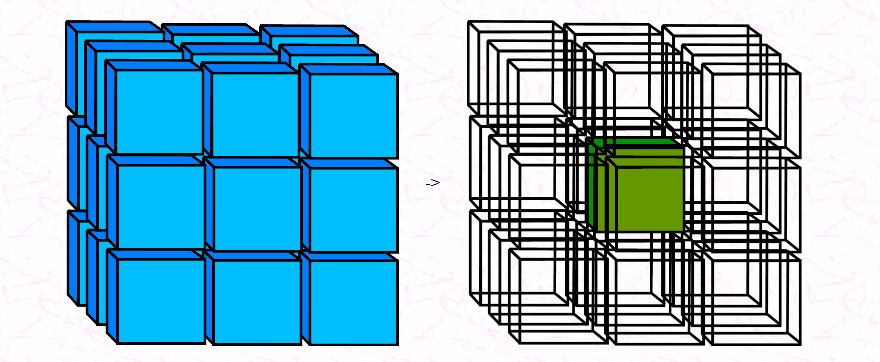
\includegraphics[width=0.8\textwidth]{imagenes/VecindadMoore.png}
                \caption[Vecindad de Moore]{Modelo de la vecindad de Moore alrededor de la celda origen}
                \label{fig:Moore}
            \end{figure}

        \subsubsection*{Integración del modelo físico de propagación}

            El paso de un voxel intacto  a una voxel en llamas sigue una adaptación estocástica del modelo físico de incendios de Rothermel (1972) aplicada a Autómatas Celulares, basándose en la formulación de Alexandridis. En este enfoque, la probabilidad de ignición ($P_{ign}$) transmitida por una celda vecina en combustión se define mediante la siguiente ecuación matemática\cite{alexandridis2008}\cite{rothermel1972}:

            $$P_{ign} = P_0 \cdot (1 + p_w) \cdot (1 + p_s) \cdot p_h$$
            \\
            Esta formulación divide la termodinámica de Rothermel en multiplicadores independientes que pueden procesarse en paralelo para millones de voxeles. Cuando una voxel que tenga la posibilidad de arder se encuentra junto a otros que ya están en  estado de fuego, el sistema procesa el riesgo de contagio evaluando cada uno de estos factores:

            \begin{itemize}
                \item \textbf{Probabilidad base y propensión del combustible ($P_0$):} Representa el tipo y la carga de combustible. Se asignan diferentes pesos según la densidad de la vegetación presente en la matriz. Por ejemplo el matorral(vegetación baja) es considerado un combustible altamente volátil que arde con rapidez por lo que va a tener una mayor propensión, mientras que el árbol (vegetación alta) tiene una mayor resistencia a la ignición, es decir, una propensión más baja.
                
                \item \textbf{Factor de viento ($p_w$):}  La influencia del viento se calcula penalizando o bonificando la probabilidad de propagación según si el viento sopla a favor o en contra de la celda y la velocidad del mismo. Se define como:
                $$p_w = \exp(V \cdot (\cos(\theta) - 1))$$
                Donde $V$ es la velocidad del viento y $\theta$ es el ángulo formado entre la dirección del viento y la línea que une el voxel en llamas con su vecino. En la implementación, este factor afecta acelerando la propagación a favor del viento y bajando la probabilidad cuando se encuentre a contraviento.

                
                \item \textbf{Factor topográfico o de pendiente ($p_s$):} Representa el ascenso del aire caliente, el cual precalienta el combustible situado cuesta arriba. Su formulación es:
                $$p_s = \exp(a \cdot \tan(\theta_s))$$
                Donde $\theta_s$ es el ángulo de inclinación del terreno. El algoritmo incrementa exponencialmente el riesgo cuando el fuego proviene de un voxel inferior, y lo penaliza en el caso contrario,cuando intenta propagarse de una delta superior a una inferior.

                
                \item \textbf{Factor de humedad ambiental ($p_h$):}  Funciona como freno general de la propagación ya que el agua contenida en la vegetación debe evaporarse antes de alcanzar el punto de ignición. Se modela como un decaimiento exponencial:
                $$p_h = \exp(-c_h \cdot H)$$
                Donde $H$ es el índice de humedad relativa (de 0 a 1) y $c_h$ es la constante de sensibilidad del combustible.

                
            \end{itemize}

            Cabe destacar el diseño estructural de la ecuación final. Los factores de viento y pendiente se añaden a la fórmula como multiplicadores de forma $(1 + p_w)$ y $(1 + p_s)$ debido a que actúan como ayudas adicionales, es decir, si las condiciones son favorables aumenta la probabilidad de propagación pero si en cambio van en contra los factores tienden a cero y el multiplicador interno queda en $1$, permitiendo que el fuego siga propagándose solo con la probabilidad base ($P_0$). \\
            
            Por el contrario, el factor de humedad ($p_h$) se aplica de forma directa porque actúa como un freno general. Si el entorno está empapado ($p_h \approx 0$), al multiplicar toda la ecuación por cero el fuego se detiene prácticamente por completo, reflejando la dinámica real de los incendios forestales.\\

            Finalmente durante la iteración de la vecindad espacial, el algoritmo suma el riesgo individual calculado de cada una de las celdas vecinas activas, dando como resultado un valor global de riesgo de ignición para la celda evaluada. Teniendo este valor de probabilidad se calcula un número aleatorio y se determina si se cambia el estado a fuego o no.\\
    
    \subsection[Visualización]{Construcción del modelo volumétrico: Raymarching y doble pase}

        Una vez que la lógica de simulación está resuelta matemáticamente el siguiente reto arquitectónico es mostrar visualmente dicha matriz tridimensional. Intentar representar con mallas cada celda en llamas colapsaría el rendimiento del sistema por lo que se ha optado por utilizar un contenedor volumétrico el cual actúa como un lienzo tridimensional encargado de interpretar la matriz térmica calculada por el \textit{Compute Shader}.\\

        Para lograr esta representación se ha implementado la técnica de \textit{Raymarching} (trazado de rayos volumétrico) que consiste en emitir un rayo virtual desde la cámara que avanza a través del interior del cubo paso a paso, muestreando en cada punto un campo de datos y asi acumular color y densidad. Para determinar la trayectoria exacta que debe recorrer cada rayo, el sistema necesita conocer exactamente en qué coordenada espacial entra el rayo al cubo (cara frontal) y en qué coordenada sale (cara trasera)\cite{gpugems3_ch30}.\\
       
        Antes de pasar a la explicación de la construcción de la escena es necesario comprender el concepto del \textit{Frame Buffer Object} (FBO).  Normalmente la GPU calcula la geometría y los shader y lo vuelca en un buffer que posteriormente se muestra por pantalla, pero al usar un FBO permite que dichos datos pasen a guardarse en la VRAM sin llegar a mostrarse por pantalla. Esto en Godot se consigue con el nodo \texttt{SubViewport} que actúa como un entorno de renderizado aislado que almacena su resultado en una \texttt{ViewportTexture} que se puede usar posteriormente.\\ 

        \begin{figure}[H]
            \centering
            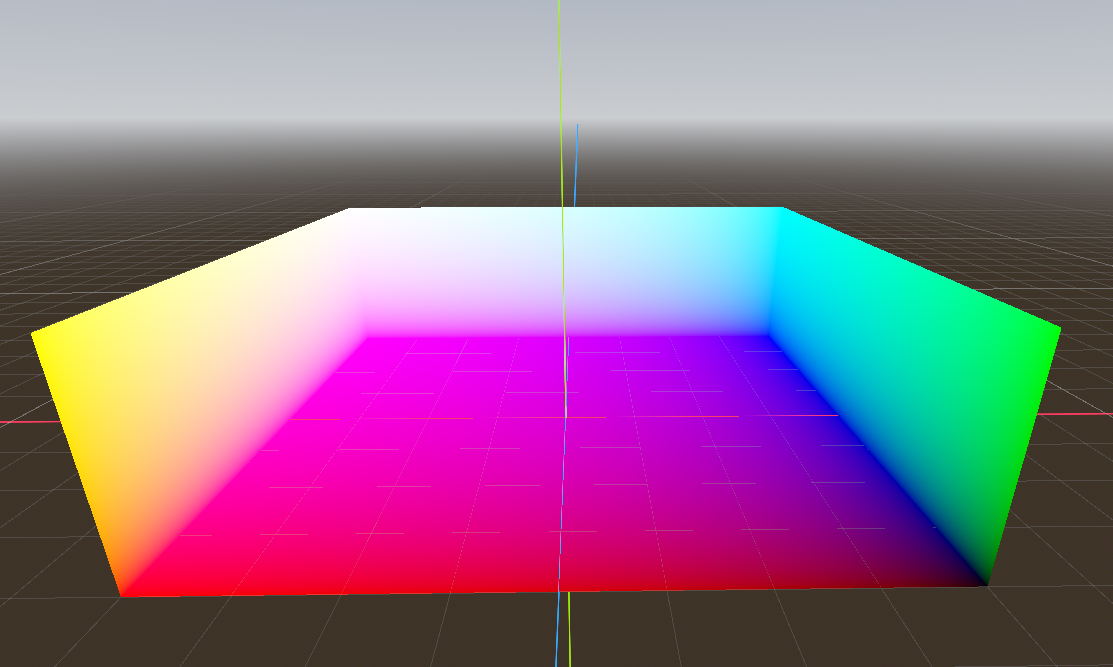
\includegraphics[width=0.6\textwidth]{imagenes/CarasTraseras.png}
            \caption[Caras traseras obtenidas por el FBO]{Vista de las caras traseras obtenidas por el FBO}
            \label{fig:CarasTraseras}
        \end{figure}
       
        \subsubsection*{Construcción de la escena y arquitectura de \textit{Shaders}}

            Para obtener estas coordenadas espaciales simultáneamente, la escena se ha estructurado utilizando un paradigma de renderizado de doble pase, el cual requiere una configuración específica de cámaras, capas de renderizado y texturas:

            \begin{itemize}
                \item \textbf{Cámaras y sincronización:} El sistema despliega dos cámaras. Una cámara principal que se encarga de registrar el movimiento del usuario e interactuar con el entorno mientras que una segunda cámara se encuentra encapsulada dentro del entorno aislado de un nodo \texttt{SubViewport} que se utilizará posteriormente para la captura de una textura. Mediante un \textit{script} en la cámara principal (y apoyado por nodos de transformación como el \texttt{RemoteTransform3D}), el sistema sincroniza la posición de ambas cámaras para que siempre muestren la misma geometría.
                
                \item \textbf{Contenedores volumétricos (Cubos):} Existen dos mallas en la escena, el \texttt{CuboFrontal} y el \texttt{CuboTrasero} (este último dentro del \texttt{SubViewport}). Para garantizar que los cálculos espaciales del rayo sean matemáticamente perfectos, ambos nodos comparten exactamente el mismo recurso de malla, asegurando que tengan la misma geometría y dimensiones en todo momento.
                
                \item \textbf{Aislamiento por capas (\textit{Cull Masks}):} Para evitar interferencias visuales entre ambos pases de renderizado, se emplea una estrategia de exclusión mediante las máscaras de capa. El \texttt{CuboFrontal} reside en la capa visual 1, mientras que el \texttt{CuboTrasero} se ubica en la capa 2. En lugar de restringir las cámaras a una única capa, se configuran para procesar todo el entorno excluyendo únicamente la capa del objeto opuesto, haciendo que la cámara secundaria tenga deshabilitada la capa 1 (ocultando así el cubo frontal), y la principal tenga deshabilitada la capa 2 (ocultando la geometría trasera). Esta configuración garantiza que cada cámara calcule exclusivamente el volumen que le corresponde sin dejar de percibir el resto de la escena.
                
                \item \textbf{Configuración de \textit{Shaders} y \textit{Render Modes}:} El núcleo de esta técnica recae en cómo la GPU procesa la superficie de estos cubos. El \texttt{CuboTrasero} posee un \textit{shader} configurado con el parámetro de renderizado \texttt{cull\_front} que obliga al motor a descartar las caras delanteras de la geometría y renderizar únicamente las caras internas (traseras). Este resultado, que contiene las coordenadas espaciales de las caras traseras, es capturado por el \texttt{SubViewport} en una textura dinámica que posteriormente es aceptada como parámetro por el shader que posee el \texttt{CuboFrontal}. Este último shader está configurado a la inversa del primero, es decir, posee el parámetro (\texttt{cull\_back}) que renderiza solo el exterior del volumen y pueda así ser usado para ejecutar el \textit{Raymarching}\cite{compute_shaders_pointclouds}.
            \end{itemize}
            
            \begin{figure}[H]
                \centering
                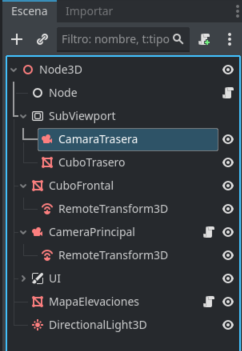
\includegraphics[width=0.5\textwidth]{imagenes/NodosGodot.png}
                \caption[Esquema de nodos de la escena]{Esquema de nodos de la escena del proyecto en Godot 4}
            \end{figure}



        \subsubsection*{Flujo técnico del renderizado de doble pase}

            El flujo técnico de este contenedor volumétrico opera de la siguiente manera:

            \begin{enumerate}
                \item \textbf{Primer pase (FBO y caras traseras):} El entorno de renderizado del  \texttt{SubViewport} utiliza una cámara interna, sincronizada con la cámara principal del usuario, y un cubo que comparte la misma malla que el cubo en la escena principal. Para renderizar únicamente las caras traseras se usa un shader que se encarga de ocultar las delanteras y ajustar la posición a un color RGB válido (de 0.0 a 1.0). Esto es necesario ya que como se mencionó anteriormente la información del \texttt{SubViewport}se guarda en una \texttt{ViewportTexture}

                \item \textbf{Segundo pase (Caras frontales y cálculo del rayo):} En la escena principal, al igual que en el \texttt{SubViewport}, se encuentran la cámara principal y el cubo frontal. Este último posee un \textit{shader} que al contrario del anterior oculta las caras traseras y lee las frontales visibles. Además acepta como parámetro la textura generada por el \texttt{SubViewport} para que por cada fragmento al restar la posición de la cara frontal a la trasera se pueda obtener el vector del rayo y saber así la dirección exacta en la que atraviesa el volumen y la distancia total de recorrido.

                \item \textbf{Avance e interpolación de la matriz (UVW):} Una vez definido el rayo, el algoritmo divide la distancia total en un bucle con un número de pasos definidos por un parámetro y con un tamaño de paso que se calcula teniendo en cuenta este número de pasos y el tamaño total del rayo. Además en cada paso, la posición local actual del rayo, que oscila entre -0.5 y 0.5, se normaliza desplazándola al rango de coordenadas de textura de 0.0 a 1.0.
                
                \item \textbf{Muestreo y acumulación de densidad:} Utilizando las coordenadas normalizadas calculadas en cada iteración del bucle, el \textit{shader} consulta el estado de ese voxel en la textura que le ha llegado como parámetro desde el \textit{Compute Shader}, donde un valor de 1.0 indica la existencia de fuego y 0.0 indica espacio vacío. Si el rayo atraviesa un voxel con fuego, se incrementa un contador el cual se usa posteriormente para calcular la densidad de ese fragmento.
                
                \item \textbf{Generación del espectro térmico:} Finalmente, con el valor de la densidad acumulada a lo largo del rayo se determina el color del píxel resultante en pantalla, para ello el sistema aplica una interpolación lineal entre colores anaranjados para las zonas de densidad baja y colores amarillos intensos para las zonas de alta densidad.
            \end{enumerate}

    \subsection[Sincronización CPU-GPU]{Comunicación y Sincronización CPU-GPU}

        Como se ha mencionado anteriormente, el costoso cálculo de la probabilidad de cada voxel para la propagación pasará a hacerse en un \textit{Compute Shader} para así aprovechar la alta capacidad de procesamiento paralelo de la GPU. Trabajar entre los dos espacios de memoria (la RAM y la VRAM) requiere una  la sincronización y transferencia eficiente de datos, que se logra de una manera más sencilla haciendo uso de la clase \texttt{RenderingDevice}.\\

        El ciclo de comunicación y ejecución de la simulación se divide en tres fases: la inyección de datos paramétricos, la sincronización de estados mediante \textit{Ping-Pong Buffers} y el despacho masivo de hilos.\\

       \subsubsection*{Inyección de datos estáticos y parámetros dinámicos}

            Antes de iniciar el cálculo de la propagación, la CPU debe preparar y transferir el contexto del entorno a la GPU. El flujo de datos se divide en dos categorías según su frecuencia de actualización: estáticos y dinámicos.\\

            Los \textbf{datos estáticos} son la topografía y el tipo de vegetación y se evalúan una única vez durante la inicialización del sistema. El \textit{script} generador del terreno recorre la matriz de elevaciones y, en función de la clasificación por colores, construye un \texttt{PackedByteArray} que se transfiere a la VRAM, donde el \texttt{RenderingDevice} lo ensambla como una textura 3D vinculada al \textit{shader}.\\
            
            \begin{lstlisting}[language=GodotShader]
            # Generacion y envio del mapa estatico (mapa_elevaciones.gd)
            func enviar_mapa_combustibles_a_gpu():
                var array_combustibles = PackedByteArray()
                array_combustibles.resize(total_celdas) 
                
                # ... (bucle tridimensional X, Y, Z) ...
                if estado == ESTADO_MATORRAL:
                    array_combustibles[indice_gpu] = 100
                elif estado == ESTADO_ARBOL:
                    array_combustibles[indice_gpu] = 255
                        
                # Se inyecta en la GPU a traves del controlador
                controlador.cargar_mapa_combustibles(array_combustibles)
            \end{lstlisting}

            Por otro lado, los \textbf{datos dinámicos} (velocidad del viento, dirección y porcentaje de humedad) se actualizan en tiempo real durante la ejecución. Para lograr esto, se hace uso de \textit{Push Constants}, una técnica que permite enviar pequeños bloques estructurados de memoria directamente a los registros ultrarrápidos de la GPU.
            
            \begin{lstlisting}[language=GodotShader]
            # Inyeccion de datos dinamicos por frame (controlador.gd)
            func ejecutar_compute_shader():
                # Empaquetamos tiempo (semilla) y meteorologia en 32 bytes exactos
                var push_constant = PackedFloat32Array([
                    semilla_cpu, 0.0, 0.0, 0.0, 
                    velViento, dir_rad, humedad, 0.0 
                ])
                var bytes = push_constant.to_byte_array()
                
                # Inyectamos en los registros de la GPU antes de ejecutar
                rd.compute_list_set_push_constant(compute_list, bytes, bytes.size())
            \end{lstlisting}

            \subsubsection*{Sincronización de estado: Técnica de \textit{Ping-Pong Buffers}}

            El modelo de propagación del autómata celular presenta un problema , si un hilo actualiza el estado de una celda de intacta a ardiendo y sobrescribe la matriz instantáneamente, los hilos que aún no hayan finalizado su ciclo leerán el dato ya modificado lo que generaría una condición de carrera que corrompería la validez del modelo.

            Para solucionar este conflicto, se implementa la técnica de \textit{Ping-Pong Buffers}, que en lugar de utilizar una única matriz, el sistema reserva dos texturas tridimensionales idénticas en la VRAM rellenándolas inicialmente con ceros que consiste en configurar un \textit{buffer} (el estado anterior) en modo de solo lectura, mientras que el segundo (el estado nuevo) como solo escritura. 
            
            \begin{itemize}
                \item \textbf{Buffer A :} Configurado en modo de solo lectura (\texttt{readonly}). Contiene la "fotografía" estática del estado actual del bosque que los hilos utilizan para evaluar a sus vecinos.
                \item \textbf{Buffer B:} Configurado en modo de solo escritura (\texttt{writeonly}). Es el lienzo en blanco donde cada hilo plasma el resultado de sus cálculos para el siguiente instante de tiempo.
            \end{itemize}

            Al finalizar cada orden de despacho computacional, la CPU invierte los punteros lógicos de ambas texturas para el siguiente \textit{frame}.
            \begin{lstlisting}[language=Python, basicstyle=\ttfamily\footnotesize, frame=single]
            # Intercambio de buffers por iteracion (controlador.gd)
            if buffer_a_es_lectura:
                rd.compute_list_bind_uniform_set(compute_list, set_a_lee_b_escribe, 0)
            else:
                rd.compute_list_bind_uniform_set(compute_list, set_b_lee_a_escribe, 0)

            # ... (Despacho a la GPU) ...

            # Preparamos el siguiente turno invirtiendo los roles
            buffer_a_es_lectura = !buffer_a_es_lectura
            \end{lstlisting}

            \subsubsection*{Configuración de \textit{Workgroups} y Despacho (\textit{Dispatch})}

            El último paso de la arquitectura es la ejecución paralela del código (\textit{Compute Shader}). El volumen no se procesa como una lista unidimensional, sino que se subdivide espacialmente para adaptarse a la arquitectura de la tarjeta gráfica y así aprovechar el paralelismo que nos ofrece.\\

            El \textit{Compute Shader} está configurado para agrupar las invocaciones en clústeres cúbicos de $8 \times 8 \times 8$ hilos por grupo. Durante la ejecución, la CPU calcula la cantidad de grupos necesarios dividiendo la resolución total de la matriz entre tamaño del \textit{Workgroup} en cada uno de sus ejes.  Finalmente, se envía el comando de despacho (\textit{Dispatch}) a la GPU que instancia simultáneamente los bloques resolviendo la propagación.\\

            \begin{lstlisting}[language=Python, basicstyle=\ttfamily\footnotesize, frame=single]
            # Division espacial y despacho concurrente (controlador.gd)
            var grupos_x = ceil(TAMANO_GRID.x / float(TAMANO_WORKGROUP.x))
            var grupos_y = ceil(TAMANO_GRID.y / float(TAMANO_WORKGROUP.y))
            var grupos_z = ceil(TAMANO_GRID.z / float(TAMANO_WORKGROUP.z))

            # Orden de ejecucion a la GPU
            rd.compute_list_dispatch(compute_list, grupos_x, grupos_y, grupos_z)
            rd.compute_list_end()
            \end{lstlisting}


\section[Topografía]{Geometría y Datos Topográficos}

    Un punto clave para un simulador de incendios es tener una buena representación del entorno para así poder conseguir resultados rigurosos.  En este proyecto, la geometría y la distribución del combustible se generan de forma procedimental a partir de Modelos Digitales de Elevaciones (DEM) y mapas satelitales de vegetación\cite{cnig_datos}.
    \subsection[Procesamiento de datos]{Procesamiento SIG, normalización y adecuación de formatos}

        Los Modelos Digitales de Elevaciones obtenidos a través de organismos oficiales se encuentran normalmente en formato GeoTIFF (\texttt{.tif}). Aunque este formato es idóneo para Sistemas de Información Geográfica (SIG), su importación directa a motores de renderizado 3D suele presentar numerosos problemas tanto en la lectura como en la precisión debido a limitaciones en la profundidad de bits por canal.\\

        Para solucionar estos problemas y garantizar un relieve topográfico y de buena fidelidad, se necesitó usar el software QGIS \cite{qgis_software}, mediante el cual los mapas originales fueron reproyectados espacialmente y delimitados al área de interés del simulador.\\ 

        Un paso crítico en esta fase fue la normalización matemática de los valores. Las cotas geográficas reales se normalizaron en un rango de 0.0 a 1.0  para que el \textit{shader} encargado de generar la elevación del terreno procese los valores como una variable de color escalar. \\

        Finalmente, el resultado es exportado al formato OpenEXR (\texttt{.exr}). Este formato, un estándar en la industria de los gráficos por ordenador, soporta valores de coma flotante lineales de 32 bits, asegurando que el mapa normalizado no sufra pérdida de precisión decimal antes de inyectarse en el motor gráfico.

    \subsection[Renderizado del terreno]{Renderizado del terreno: Desplazamiento y normales}

        Una vez procesados, los mapas se integran en el simulador. La representación visual no emplea una malla estática, sino que parte de un plano base que es deformado mediante un \textit{shader} espacial (\texttt{spatial})\cite{escudero2023}.\\

        Este \textit{shader} se encarga de alterar la coordenada vertical de cada vértice muestreando el mapa de elevaciones introducido.Posteriormente, el valor normalizado leído se multiplica por el diferencial real de altura del terreno, obteniendo así la elevación exacta del relieve original.\cite{heightmap}\\

       \begin{lstlisting}[language=C, basicstyle=\ttfamily\footnotesize, frame=single]
        // Lectura y desplazamiento geometrico de la orografia (Shader)
        void vertex() {
            // Lectura de la altitud normalizada (0.0 a 1.0) en el mapa OpenEXR
            float altura_leida = textureLod(mapa_elevacion, UV, 0.0).r;

            // Proteccion matematica contra pixeles corruptos (NaN/Inf)
            float altura_segura = (isinf(altura_leida) || isnan(altura_leida)) 
                                ? altura_base : altura_leida;

            // Decodificacion: Desplazamiento 3D escalar del vertice
            VERTEX.y += (altura_segura - altura_base) * escala_altura;
            
        }
        \end{lstlisting}


        Un problema generado por alterar los vértices de forma dinámica es que los vectores normales originales del plano dejan de ser válidos, lo que provoca que no se calcule correctamente las sombras y la iluminación. Para solucionarlo, el \textit{shader} recalcula la inclinación real del terreno leyendo la altitud de los cuatro píxeles vecinos y construyendo dos vectores direccionales (el vector tangente y el vector binormal) cuya diferencia angular conforma la pendiente\cite{foley2014computer}.\\
        
        \begin{figure}[H]
            \centering
            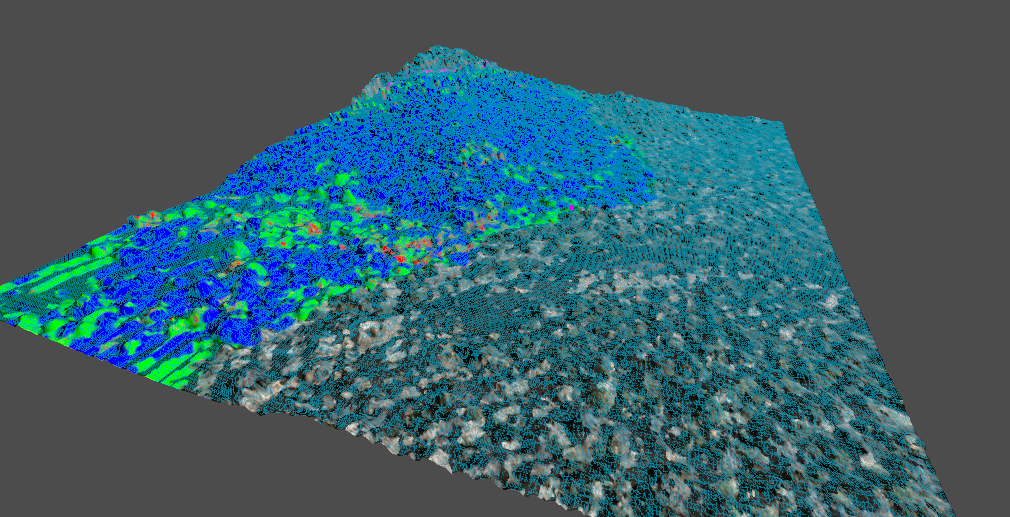
\includegraphics[width=0.8\textwidth]{imagenes/MapaElevaciones.png}
            \caption[Mapa generado por un DEM]{Mapa generado a partir de un Modelo Digital de Elevaciones}
            \label{fig:MapaElevaciones}
        \end{figure}

        Finalmente, el \textit{shader} le asigna el color leyendo el mapa satelital de vegetación y ajustando los parámetros físicos del material (\texttt{ROUGHNESS} y \texttt{SPECULAR}) para simular la reflexión lumínica parecida a la de la realidad.

    \subsection[Construcción de la matriz lógica]{Extracción a memoria principal y discretización volumétrica}

        Para construir la matriz lógica del autómata celular, la CPU extrae, descomprime y redimensiona las texturas visuales hacia la memoria RAM. Este volumen espacial se estructura en un (\texttt{PackedInt32Array}) para obtener un mejor rendimiento y se procesa siguiendo un proceso:
        \begin{enumerate}
            \item \textbf{Cálculo espacial:} Lee el píxel del mapa de elevaciones y lo multiplica por la resolución vertical del contenedor volumétrico para calular índice exacto de la superficie.
            \item \textbf{Análisis del color vegetal:} Analiza los canales RGB del píxel. Si el espectro azul es dominante, se almacena como vegetación alta (\texttt{ESTADO\_ARBOL}), si predomina el rojo, vegetación baja (\texttt{ESTADO\_MATORRAL}) y el resto de valores se asume como terreno que no puede incendiarse (\texttt{ESTADO\_SUBSUELO})
        \end{enumerate}

        Finalmente, el algoritmo rellena verticalmente los voxeles inferiores al que contiene la vegetación como voxeles con estado (\texttt{ESTADO\_SUBSUELO})


\section{Interacción y Control Dinámico}
Para que el simulador sea accesible y permita al usuario visualizar la escena desde distintos ángulos e interactuar con los factores de simulación se han desarrollado una serie de mecanismos y elementos en Godot.
 
    \subsection[Generación de colisiones]{Generación de colisiones topográficas}

        El renderizado de la simulación volumétrica y el \textit{shader} que genera el desplazamiento topográfico de las elevaciones no poseen una malla para el subsistema de colisiones de Godot, impidiendo que se pueda interactuar con el terreno mediante el ratón.
        
        Para solucionar esto se ha generado una  \texttt{HeightMapShape3D} que es un  componente que construye dinámicamente un campo de alturas sólido superpuesto a la representación visual. Los valores de altitud originales se ponderan por el factor de diferencia escalar y se ajustan a las cotas límite del mundo. Una vez calculada esta malla de colisión  se pueden llevar a cabo los (\textit{RayCasts}) emitidas desde la cámara del usuario para desencadenar la ignición inicial del incendio de forma precisa e interactiva.
    
    \subsection[Navegación espacial]{Navegación espacial y cámara libre}
    La simulación cuenta con un sistema de cámara de vuelo libre, que permite al usuario desplazarse sin restricciones espaciales por la escena, utilizando un control clásico mediante teclado y ratón.\\ 
    
    La capacidad de observar la propagación de las llamas desde cualquier punto resulta de gran utilidad ya que permite ver en detalle cómo el fuego interactúa con pendientes y tipos de vegetación específicos y obtener asi una perspectiva del alcance general de la emergencia.

    \subsection[Sistema de Ignición]{Sistema de Ignición: Interacción espacial y traducción}

        Además de la visualización de con el movimiento de la cámara se ha implementado un sistema (\textit{RayCast}) que interactúa con la malla de colisión generada para el terreno y que nos permite iniciar el incendio en cualquier punto de la topografía.\\

        Al registrarse el clic de ignición, el motor proyecta un rayo desde el origen de la cámara en movimiento hacia el mundo físico. Si este rayo intersecta con la malla de colisión topográfica generada anteriormente, el algoritmo recupera el punto de impacto global.\\

        \begin{lstlisting}[language=Python, basicstyle=\ttfamily\footnotesize, frame=single]
        # Lanzamiento del rayo de interaccion (mapa_elevaciones.gd)
        var centro_pantalla = get_viewport().get_visible_rect().size / 2.0
        var origen = camara.project_ray_origin(centro_pantalla)
        var direccion = camara.project_ray_normal(centro_pantalla)

        # Proyeccion e interseccion fisica
        var impacto = espacio_fisico.intersect_ray(parametros_rayo)
        \end{lstlisting}
        

        Debido a que la matriz topográfica opera en un espacio local, la coordenada global del impacto debe ser traducida al sistema de referencia del volumen contenedor. Primero normaliza los vectores para evitar desfases de escala, y seguidamente el algoritmo calcula los índices matemáticos discretos (X, Z) multiplicando la posición local por la resolución base de la matriz. \\

        \begin{lstlisting}[language=Python, basicstyle=\ttfamily\footnotesize, frame=single]
        # Traduccion a matriz y encendido espacial (mapa_elevaciones.gd)
        var pos_local = cubo_frontal.to_local(punto_global)
        var pos_normalizada = pos_local + Vector3(0.5, 0.5, 0.5)

        # Calculo del indice matricial (X, Z)
        var x_matriz = int(pos_normalizada.x * resolucion.x)
        var z_matriz = int(pos_normalizada.z * resolucion.z)

        # El controlador actualiza la VRAM con el nuevo foco
        controlador.agregar_fuego_en(x_matriz, y_matriz, z_matriz)
        \end{lstlisting}

    \subsection[Interfaz de Usuario]{Interfaz de Usuario y Control Meteorológico}

    En un entorno real durante un incendio los factores ambientales no son estáticos sino que cambian a lo largo del tiempo que dura el incendio. En el simulador se ha logrado esto mediante una  Interfaz de Usuario (UI) superpuesta al visor volumétrico.\\

    Dicha interfaz tiene varios \textit{sliders} representando la velocidad del viento, dirección del viento (en grados) y el índice de humedad. Estos \textit{sliders} están vinculados mediante señales al \textit{script} principal del controlador por lo que cualquier modificación realizada por el usuario es capturada instantáneamente.\\
    \begin{figure}[H]
        \centering
        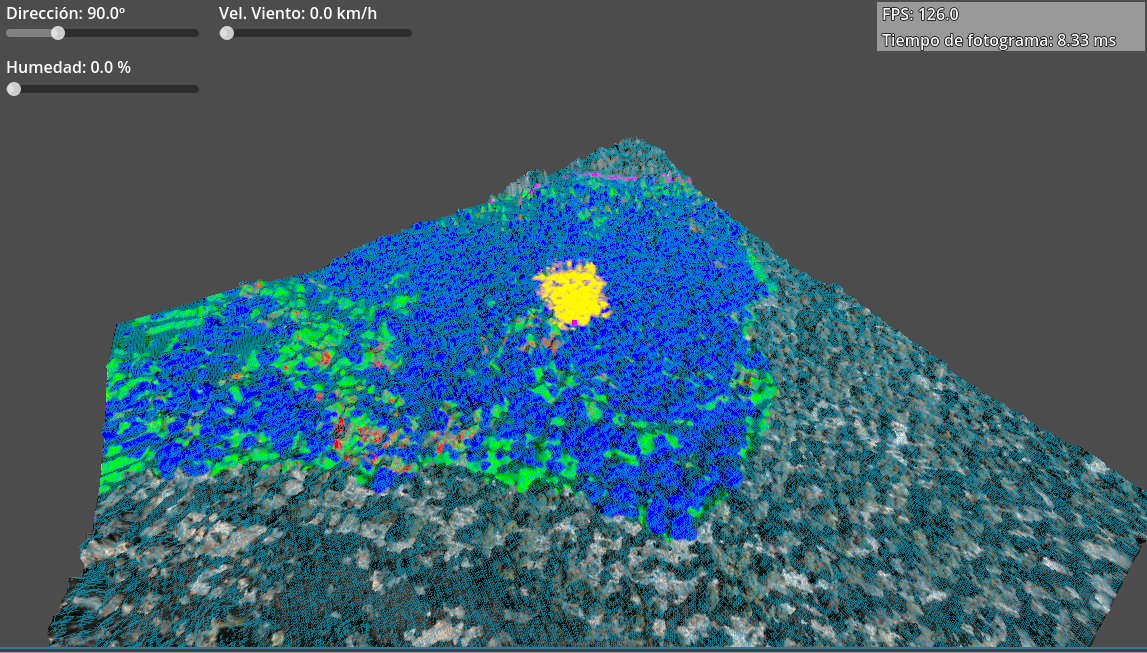
\includegraphics[width=0.8\textwidth]{imagenes/InterfazUI.png}
        \caption{Interfaz de Usuario del simulador}
        \label{fig:UI}
    \end{figure}

    Dado que estos parámetros se envían a la tarjeta gráfica empaquetados como \textit{Push Constants} en cada ciclo de iteración, el cambio en las condiciones del entorno tiene un efecto inmediato en el \textit{Compute Shader}, lo que permite observar cómo las llamas se adaptan a las nuevas variables sin necesidad de pausar, recalcular o reiniciar la simulación.\\

\section{Desafíos Técnicos y Soluciones}

    El desarrollo de este simulador ha supuesto diversos retos arquitectónicos y matemáticos. A continuación, se detallan los desafíos más significativos encontrados durante la implementación y las soluciones aplicadas para resolverlos.\\

    \subsection[Optimización del \textit{Raymarching}]{Optimización del \textit{Raymarching} mediante Salida Temprana}
        \textbf{El problema:} 
        La técnica de \textit{Raymarching} tiene un alto coste computacional. Para una resolución de pantalla estándar (1080p), emitir un rayo por cada píxel y hacerlo dar un gran número de  pasos implicaba ejecutar decenas de millones de lecturas a la textura 3D por cada \textit{frame}. Inicialmente, se evaluaba el rayo completo incluso cuando atravesaba zonas densas de fuego o zonas completamente vacías, provocando bajos fotogramas por segundo (FPS).\\

        \textbf{La solución:} 
        Se implementó una estrategia algorítmica de salida temprana en la que en \textit{shader} de la segunda pasada, se estableció un umbral para la densidad acumulada. Al alcanzar este umbral el bucle se interrumpe eliminando los cálculos innecesarios en las regiones internas y posteriores del fuego, y estabilizando el rendimiento en tiempo real.
        \\


        \begin{lstlisting}[language=C, basicstyle=\ttfamily\footnotesize, frame=single]
        // Optimizacion de salida temprana (TwoPassRendering.gdshader)
        densidad_acumulada += (densidad_punto * multiplicador) * tamano_paso;

        if (densidad_acumulada >= 1.0) {
            break; // El rayo no necesita seguir avanzando
        }
        \end{lstlisting}

    \subsection{Sincronización de Espacios de Coordenadas}

    \textbf{El problema:} 
    El sistema de ignición interactiva presentaba una desincronización espacial. Al realizar un clic sobre una montaña, el fuego aparecía en ubicaciones incorrectas o fuera de los límites de la matriz. Esto ocurría porque no se estaban haciendo correctamente los cambios entre los tres espacios matemáticos, las coordenadas globales del motor físico, las coordenadas locales del cubo contenedor y el índice discreto de matriz del autómata celular.

    \textbf{La solución:} 
    Se desarrolló un flujo de traducción de coordenadas secuencial. Primero, el punto de impacto global devuelto por el \textit{RayCast} se transforma al espacio local del contenedor. Debido a que las coordenadas de la malla se encuentran entre -0.5 y 0.5, se le suma un vector \texttt{(0.5, 0.5, 0.5)} para obtener coordenadas normalizadas estrictamente positivas entre 0.0 y 1.0. Finalmente, este valor decimal se multiplica por la resolución máxima de la matriz del autómata 

    \subsection[Anomalías en el Relieve]{Anomalías Geométricas en la Generación del Relieve}
    \textbf{El problema:} 
    Durante las primeras pruebas de importación de los mapas de elevaciones (DEM), el desplazamiento de los vértices en el \textit{shader} generaba columnas gigantes y picos que no coincidían con la topografía real. Investigandolo se descubrió que este fallo se originaba por dos factores. En primer lugar, los datos del DEM representaban altitudes reales en metros que producían un desbordamiento que disparaba los vértices fuera de los límites de renderizado. En segundo lugar, al recortar las regiones de interés en QGIS, algunos píxeles se exportaban con valores nulos (\texttt{NaN}), o infinitos (\texttt{Inf}).\\

    \textbf{La solución:} 
    Para solucionar el primer problema se optó por la normalización de la textura en QGIS. Mediante el uso de álgebra de mapas, todas las cotas se remapearon a un rango de 0.0 a 1.0, permitiendo que el desplazamiento de vértices usando un escalado para la altura de como resultado una visualización correcta. 

    Para el segundo problema se aplicó directamente un filtro en el \textit{shader} que se encarga de evaluar las alturas leídas de la textura normalizada mediante las funciones nativas \texttt{isinf()} e \texttt{isnan()}. Si el píxel es nulo o infinito, fuerza su altitud a la altura base.\\


    \begin{lstlisting}[language=C, basicstyle=\ttfamily\footnotesize, frame=single]
    // Proteccion matematica contra pixeles corruptos
    float altura_leida = textureLod(mapa_elevacion, UV, 0.0).r;

    // Si la imagen EXR tiene errores (Infinito o NaN), forzamos la altura base
    float altura_segura = (isinf(altura_leida) || isnan(altura_leida)) 
                        ? altura_base : altura_leida;

    // Desplazamiento 3D proporcional tras la normalizacion en QGIS
    VERTEX.y += (altura_segura - altura_base) * escala_altura;
    \end{lstlisting}

    \subsection[Desincronización de Cámaras]{Desincronización de Cámaras en el Contenedor Volumétrico}

    \textbf{El problema:} 
    Cuando el usuario utilizaba la cámara libre para moverse por el escenario ocurrían varios errores en la visualización del fuego, como que el volumen del fuego aparecía cortado o que flotaba fuera de su posición. Tras investigarlo se descubrió que el origen del error se daba en la técnica de doble pase, más concretamente en la sincronización de las posiciones. Para que el cálculo del vector del rayo sea correcto la cámara secundaria del \texttt{SubViewport} debe observar el cubo desde el mismo ángulo exacto que la cámara principal.

    \textbf{La solución:} 
    Para solucionar estos errores se desarrolló un \textit{script} que garantiza que al inicio de la simulación la cámara secundaria copie los parámetros de proyección de la cámara principal, es decir, el \textit{FOV}, el \textit{Near} y el \textit{Far}.
    
    Por otro lado, se usó un nodo que proporciona Godot, el  (\texttt{RemoteTransform3D}), sobre la cámara principal vinculandolo con la cámara del \texttt{SubViewport}. Este nodo se encarga de que la cámara secundaria replique continuamente la posición, rotación y escala de la principal.

    Al sincronizar perfectamente ambas cámaras, las coordenadas de textura proyectadas en el \texttt{SubViewport} coinciden sin errores, haciendo que se visualice correctamente desde cualquier ángulo y distancia.




\section{Integración y uso de Inteligencia Artificial}

    Durante el desarrollo de este proyecto, se ha hecho uso de modelos de Inteligencia Artificial (IA) generativa, concretamente \textbf{Gemini} apoyado por \textbf{Claude} para las labores específicas de programación, como asistentes para diversas tareas. El uso de esta tecnología se ha planteado desde un punto de vista instrumental, como una herramienta más, con el objetivo de optimizar los tiempos de aprendizaje, resolución de problemas y redacción, manteniendo en todo momento la autoría, el diseño arquitectónico y el criterio técnico sobre el resultado final.\\

    Al enfrentarse a una curva de aprendizaje pronunciada con herramientas complejas nunca antes vistas, como el motor de desarrollo Godot 4 o el software de información geográfica QGIS, Gemini ha actuado como un tutor interactivo acelerando la comprensión de los flujos de trabajo de los entornos y las herramientas que estos ofrecían. Por otro lado, uno de los mayores retos del proyecto fue orquestar una comunicación eficiente entre la memoria del sistema (RAM) y la memoria de vídeo (VRAM). En este ámbito analítico, Claude sirvió como soporte de consulta para entender a bajo nivel el funcionamiento de la clase \texttt{RenderingDevice}, asimilar los conceptos de despacho concurrente en los \textit{Compute Shaders} y agilizar la escritura de código y depuración de dicha sincronización.\\

    A su vez, la representación visual de la matriz térmica mediante el contenedor volumétrico supuso un gran desafío técnico durante sus etapas iniciales debido a los errores que iban apareciendo. En este contexto de desarrollo, la IA demostró ser un recurso muy eficaz para el escrutinio de código y el diagnóstico rápido de fallos, permitiendo aislar y corregir de forma ágil los distintos \textit{bugs} y anomalías visuales que corrompían la imagen, acelerando así la corrección de los \textit{shaders} hasta alcanzar la fidelidad visual buscada en el simulador.\\

    Finalmente, para la elaboración de esta memoria, Gemini ha desempeñado un papel fundamental como asistente para la estructuración y revisión de estilo de la misma. Se empleó principalmente para perfilar la estructura lógica de los capítulos, afianzar el rigor formal exigido en el ámbito universitario y facilitar el formateo del texto y las fórmulas matemáticas mediante \LaTeX. En definitiva, la inteligencia artificial ha actuado como un recurso complementario que ha agilizado significativamente todas las fases del trabajo. No obstante, la validación de los modelos físicos, las decisiones de ingeniería de software y la implementación final del sistema han dependido exclusiva y estrictamente del criterio del autor.\\



